In this section, the Database Layer is described in some detail n terms of its specific subsystems.

\subsection{Database Tables}
The Database Tables Subsystem is what provides the database with all the needed information for the website. This data is connected through HTML and PHP code to gather information from the tables or even put data back into the tables properly. This allows for proper storage of information to the database so that the website portion may run smoothly and without any error or incorrect information when sought by a user.

\begin{figure}[h!]
	\centering
 	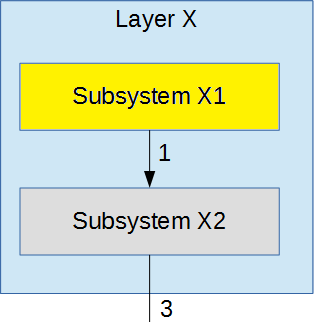
\includegraphics[width=0.60\textwidth]{images/subsystem}
 \caption{Example subsystem description diagram}
\end{figure}

\subsubsection{Assumptions}
The main assumption concerning the Database Tables was that it was an important part of the project to run efficiently.

\subsubsection{Responsibilities}
The Database Tables were a significant portion of the project. It stores everything needed for the actual website to display some sort fo information without hard coding data into fields. The Database Tables needed to be correct and also be connected to one each other to extract information from multiple tables and make sure that the information needed was the correct information that is being sent. This ensured any communication with the website server and database went successfully and provided the correct info needed.

\subsubsection{Subsystem Interfaces}
Each of the inputs and outputs for the subsystem are defined here. Create a table with an entry for each labelled interface that connects to this subsystem. For each entry, describe any incoming and outgoing data elements will pass through this interface.

\begin {table}[H]
\caption {Subsystem interfaces} 
\begin{center}
    \begin{tabular}{ | p{1cm} | p{6cm} | p{3cm} | p{3cm} |}
    \hline
    ID & Description & Inputs & Outputs \\ \hline
    \#1 & CREATE DATABASE & \pbox{3cm}{Name of Database} & \pbox{3cm}{Database is created with given input name}  \\ \hline
    \#2 & CREATE TABLE & \pbox{3cm}{Name of Table} & \pbox{3cm}{Table is created in current Database}  \\ \hline
    \#3 & INSERT TO and VALUES & \pbox{3cm}{Table's Column's Names and Values} & \pbox{3cm}{Information filled tables}  \\ \hline
    \end{tabular}
\end{center}
\end{table}
